%TC: macro \marginfootnote [other]
%TC: envir SCfigure [] other
%TC: macrocount beginSCfigure [figure]
\documentclass[11pt,twoside]{report}
\usepackage{preamble}
\setcounter{chapter}{5}
\graphicspath{{../img/}}
\def\includebibliography{}

\begin{document}
\chapter{Nucleation kinetics in simple drying aerosols}
\epigraph{Remove the plastic.}{Sears\textsuperscript{\textregistered} cross-trainer manual.}
\label{chapter:aerosols}

In previous chapters we have focused on modelling hard spheres at high densities, with a particular focus on supercooled liquids and glasses.
As we mentioned in the introduction, another central topic of the high density liquid is the nucleation process by which the liquid becomes a crystal.
This chapter addresses nucleation within the context of drying aerosol droplets, with applications to climate modelling and industrial spray drying.
The chemistry involved makes this system much more complicated than can be captured with a simple hard sphere interaction, so our microscopic morphometric formalism will not work here at present.
Instead we will start from the mesoscale limit, where the droplet can be treated as a continuum.
%% At present real systems are too complex to be treated from first principles, so we will employ phenomenological fits to available data assuming classical nucleation theory.
%% We hope one day theory will allow a connection between microscopic and mesoscopic approaches, paving the way to a properly first-principles treatment of real systems.

This work was undertaken in collaboration with members of the Reid group in the School of Chemistry at the University of Bristol.
In particular, the experiments were carried out by Flo Gregson.
My contribution to this work was through theory and numerical modelling to better understand the experimental data.
Consequently, while I will describe the experiments the focus of the chapter will be theoretical.
Some of this work has already been published in Ref.\ \cite{GregsonJPCB2019}, and we hope to publish the remainder in Refs.\ \cite{RobinsonTBD2019,GregsonTBD2019} later this year.

\section{Introduction}

The impact of atmospheric aerosols on the climate remains the leading single uncertainty in climate predictions \cite{BoucherIPCC2013,CarslawN2013,LeePNAS2016,RegayreACP2018}.
In particular, the radiative forcing caused by anthropogenic aerosols in clouds features large uncertainties due to the difficulty of direct measurement, and the large parameter spaces of theoretical models \cite{LeePNAS2016}.
Thus, the importance of improving models for atmospheric aerosols to better predict climate change and inform policy cannot be overstated.
In addition, atmospheric aerosols have potential applications in geoengineering \cite{PringleACP2012}.

Notably, radiative forcing of atmospheric aerosols is stongly influenced by their optical properties \cite{HodasACP2015,CotterellACP2017}.
The solute concentration and physical state (i.e.\ whether it is crystalline or amorphous) can thus have a dramatic effect on climate predictions.
Central to this is the nucleation and drying kinetics of atmospheric droplets.
Where aerosols are included in climate models the focus is typically on sulphates \cite{MannACP2014,ZhuNC2019}.
However, sea salt aerosols (e.g.\ those containing \ce{NaCl}), deposited into the atmosphere through natural processes, are more prevalent in the atmosphere than sulphates making up the second largest component of atmospheric aerosols by mass \cite{KeeneJAS1998}; a major component of aged \ce{NaCl} aerosols is sodium nitrate (\ce{NaNO3}) formed through reactions with nitrogen oxides \cite{TolockaJPCA2004}, a significant industrial emission.
Subsequent reactions form secondary organic aerosols which further impact the climate \cite{ScottACP2014,PoschlCR2015} and are associated with adverse health effects \cite{PoschlCR2015}.
Given their abundance and relative simplicity we focus on \ce{NaCl} and \ce{NaNO3} aerosol droplets.

Understanding the droplet drying and crystallisation process is also important for industrial applications, most notably in spray-drying.
The goal in these applications is to control the distribution of sizes, morphology and phase of the final droplets, which are very sensitive to processing conditions such as solvent \cite{CarverIECR2012,LintingreSM2016}, temperature \cite{IveyAST2018,YouDT2014,LinPT2015}, pH \cite{YuJPS2002,DubbiniIJP2014} and additional co-excipients \cite{ZhongAP2018,NandiyantoAPT2011,LyuJCG2017}.
Tailoring crystallisation is particularly important because crystal and amorphous states have fundamentally different properties: crystalline droplets are typically more stable, suitable for e.g.\ product storage \cite{VehringJAS2007,CostantinoJPS1998}, whereas amorphous droplets are more soluble which is desirable for e.g.\ drug delivery \cite{AmstadJPCB2016,BroughIJP2013}.
Our investigation of crystal nucleation rates can be inverted to design spray-drying conditions to achieve a desired final state.

In this chapter we will investigate drying and crystal nucleation of free aerosol droplets, by combining experiments and a numerical model of free aerosol droplets.
The experiments are described in section \ref{sec:experiments}, and we report matching them to a diffusional model of droplet evolution in section \ref{sec:evolution}.
We find that classical nucleation theory accurately predicts the crystallisation times for \ce{NaCl} aerosols, but not for \ce{NaNO3}, in section \ref{sec:nucleation}.
For \ce{NaNO3} we report nucleation rates with non-monotonic behaviour with increasing solute concentration.

\section{Experiments}
\label{sec:experiments}

The kinetics of drying \ce{NaCl} and \ce{NaNO3} droplets was measured using the Comparative-Kinetics Electrodynamic Balance (CK-EDB).
In all experiments HPLC-grade water, BioXtra $\ge 99.5\%$ \ce{NaCl} (Sigma-Aldrich) and analytic grade \ce{NaNO3} (Fisher-Scientific) were used.
The CK-EDB instrument has been detailed in previous work \cite{DaviesAST2012} so we will only describe it briefly here.
Droplets of known concentration are produced by a droplet-on-demand generator (MicroFab) and injected into the CK-EDB instrument.
Upon generation the droplets are charged ($<\SI{10}{\femto\coulomb}$ through e.g.\ an ionic imbalance) with an induction electrode such that they become trapped within the centre of the electrodynamic field, produced by the application of an AC field between two sets of concentric cylindrical electrodes.
An additional DC field is applied to the lower set of electrodes to counteract gravity and drag forces acting on the droplet.
A circulating current of ethylene glycol coolant across the electrodes controls the chamber temperature $T_{\infty}$ in the range 273--\SI{323}{\kelvin}.

To determine the size and physical state of the droplet, it is illuminated with a \SI{532}{\nano\metre} continuous-wave laser.
The resulting scattering pattern is recorded by a CCD camera placed at \SI{45}{\degree} to the beam over an angular range of $\SI{\sim24}{\degree}$.
For isotropic droplets in a liquid or dried amorphous state the droplet radius $R$ determines the angular separation between the fringes in the pattern $\Delta \theta$.
Assuming the geometric optics approximation of Mie theory, this relationship is given by
\begin{equation*}
  R
  =
  \frac{\lambda}{\Delta \theta} \left(
  \cos{\left(\frac{\theta}{2}\right)}
  + \frac{n \sin{\left(\frac{\theta}{2}\right)}}{\sqrt{1 + n^2 - 2n \cos{\left(\frac{\theta}{2}\right)}}}
  \right)^{-1}
\end{equation*}
where $\lambda$ is the laser wavelength, $\theta$ is the central viewing angle and $n$ is the droplet refractive index.
This approximation scheme determines the droplet radius within an accuracy of $\SI{\pm100}{\nano\metre}$.
This method fails when crystallisation occurs breaking isotropy and the scattering pattern dramatically changes; this feature allows the time of crystallisation to be determined to within $\SI{\sim10}{\milli\second}$.
Nucleation and growth occur on such a short time scale that it is not possible to obtain information from the experiments on where inside the droplet this occurs or how many initial nucleation sites there were; we can only determine that the droplet has nucleated crystals.

The instrument features two gas flows for wet and dry nitrogen applied to the droplet at a rate of \SI{0.03}{\metre\per\second}.
Controlling the ratio of these two flows through a mass-flow controller (MKS instruments) sets the relative humidity (RH) inside the CK-EDB chamber.
Liquid aqueous \ce{NaCl} and aqueous \ce{NaNO3} droplets (20\% solute concentration by weight) were evaporated into dry conditions at \SI{20}{\celsius}.
Crystallisation of multiple \ce{NaCl} droplets occurred reproducibly \SI{1}{\second} after droplet generation \cite{GregsonJPCB2019}, whereas \ce{NaNO3} droplets showed stochastic behaviour with a fraction of droplets not crystallising over the timescale of the experiment (droplets were typically trapped for \SI{10}{\second}).
The stochastic behaviour persists when the experiment was repeated for the \emph{same} \ce{NaNO3} droplet over a cycle of repeatedly lowering and raising the RH (described in more detail in Ref.\ \cite{GregsonTBD2019}), ruling out impurity-driven heterogeneous nucleation.

\begin{SCfigure}
  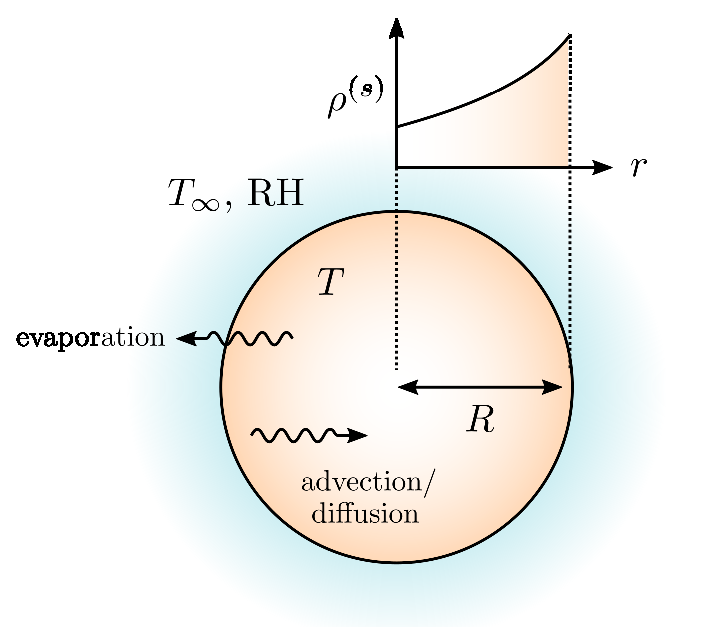
\includegraphics[width=0.75\linewidth,outer]{aerosol-droplet}
  \caption[Model drying aerosol droplet]{
    A drying droplet solution of radius $r=R(t)$ surrounded by a gas of temperature $T_\infty$ and relative humidity RH.
    Evaporation of the solvent (water) causes the droplet to shrink and surface enrichment of solute concentration $\rho^{(s)}$ together with evaporative cooling $T < T_\infty$.}
  \label{fig:aerosol-droplet}
\end{SCfigure}

Follow up experiments by the Reid group placed the droplets inside a scanning electron microscope (SEM) for imaging.
These found that for \ce{NaCl} aerosols nucleation seems to occur at the boundary%
\marginfootnote{I am reversing chronology here: actually, we used our numerical model to predict this \emph{first}, which was then was confirmed by SEM images.}.
The experiments featuring slower evaporation tended to have more perfect crystals suggesting there were fewer nucleation sites, whereas the more rapidly evaporating droplets showed imperfections consistent with there being multiple nucleation sites at the boundary \cite{GregsonTBD2019}.
The SEM results for \ce{NaNO3} were inconclusive, although the resulting crystals were more spherical suggesting there were multiple nucleation sites which may be less strongly distributed at the boundary.

\section{Model for a drying droplet}
\label{sec:evolution}

\subsection{Overview and notation}

In order to obtain nucleation rates we require the time evolution of the droplet's concentration profile over its drying history, and a phenomenological model for nucleation rates based on concentration.
To determine the concentration profile trajectory for a drying droplet we have to consider the relative motion of solute and solvent species inside the droplet, of various species in the surrounding vapour phase, as well as the evaporation of solvent across the phase boundary.
Our approximations will reduce this to a moving boundary problem with solely diffusional mixing.

Prior to crystallisation a drying droplet will be approximately spherical, so we consider a phase boundary at radius $R(t)$ evolving in time $t$.
Writing the distance from the center of the droplet as $r$, the phase boundary separates the liquid phase inside $r \in [0, R(t))$ from the vapour phase outside $r \in (R(t), \infty]$.
The droplet is sketched in Fig.\ \ref{fig:aerosol-droplet}.
%In the experiments are performed in ambient conditions so the surrounding gas is strictly speaking a mixture, but to a reasonable approximation we can treat it as a single component.

We label the solute and (ambient) gas components as $s$ and $g$ respectively, and the evaporating solvent component as $f$ for \emph{fluid} as it exists in both the liquid and gas phases.
The density is $\rho = \sum_i \rho^{(i)}$ where the (mass) concentration of each component is $\rho^{(i)}$ for $i \in (f,s)$ in the droplet and $i \in (f,g)$ in the gas.
A useful auxillary variable is the mass fraction of each component, i.e.\
\begin{equation}\label{eq:mass-fraction}
  Y^{(i)} = \frac{\rho^{(i)}}{\rho}.
  %{\sum_j \rho^{(j)}}
  %{\rho^{(f)} + \rho^{(s)}}
  %\frac{\rho^{(i)}(\vec{r})}{\rho^{(f)}(\vec{r}) + \rho^{(s)}(\vec{r})}
  %\qquad i \in \{f, s\}.
\end{equation}
%with $j$ running over the components of the relevant phase.
%Clearly $Y^{(f)} = 1 - Y^{(s)}$
As both phases are binary mixtures%
\marginfootnote{This is not strictly true.
  The liquid phase is certainly a binary mixture of solvent and solute, however the vapour is composed of the evaporated solvent and a multicomponent ambient gas phase.
  However, we can treat the ambient gas as an effectively single-component system to a very good approximation.}
so we only need to solve for one component; we choose to solve for the solute mass fraction $Y^{(s)}$ in the droplet and the solvent mass fraction $Y^{(f)}$ in the surrounding vapour.

The thermal conductivity of liquids is generally much larger than the mass diffusivity, so to leading order we can treat temperature $T$ as homogeneous throughout the droplet.
This approximation neglects potential conduction forces driven by temperature gradients.
The droplet temperature will be smaller than the ambient temperature $T_\infty$ because vaporisation carries a latent heat
We will determine $T$ through the rate of vaporisation which will be moderate the vaporisation rate and enter into the nucleation calculations.
However, as a simplification we do not incorporate this temperature into the dynamics themselves through modified diffusion coefficients.

\subsection{Evolution of the concentration profile}

In the absence of any chemical reactions the continuity equation for each species component reads
\begin{equation}\label{eq:species-continuity}
  \frac{\partial \rho^{(i)}}{\partial t} +
  \vec{\nabla} \cdot (\rho^{(i)} \vec{v}^{(i)}) = 0
  \qquad i \in \{f,s\}
\end{equation}
where $\vec{v}^{(i)}$ is the velocity of species $i$, or in terms of relative flows
%% and the mass-averaged fluid velocity is
%% \begin{equation}
%%   \vec{v} = \sum_i Y^{(i)} \vec{v}^{(i)}
%% \end{equation}
%% We have
%% \begin{equation*}
%%   \frac{\partial \rho^{(i)}}{\partial t} +
%%   \vec{\nabla} \cdot (\rho^{(i)} \vec{v}) +
%%   \vec{\nabla} \cdot (\rho^{(i)} (\vec{v}^{(i)} - \vec{v})) = 0
%%   \qquad i \in \{f,s\}
%% \end{equation*}
%% and defining the relative mass flux as
%% \begin{equation}\label{eq:relative-mass-flux}
%%   \vec{j}^{(i)} = \rho^{(i)} (\vec{v}^{(i)} - \vec{v})
%%   \qquad i \in \{f,s\}
%% \end{equation}
%% gives
\begin{equation}\label{eq:species-continuity-relative}
  \frac{\partial \rho^{(i)}}{\partial t} +
  \vec{\nabla} \cdot (\rho^{(i)} \vec{v}) +
  \vec{\nabla} \cdot \vec{j}^{(i)} = 0
  \qquad i \in \{f,s\}
\end{equation}
where the mass-averaged fluid velocity is $\vec{v} = \sum_i Y^{(i)} \vec{v}^{(i)}$ and the relative mass flux is $\vec{j}^{(i)} = \rho^{(i)} (\vec{v}^{(i)} - \vec{v})$.
Any advective/convective flows will typically be contained in $\vec{v}$, while diffusive effects are captured by $\vec{j}^{(i)}$.

Volume additivity holds to a good approximation \cite{HandscombCES2009}, i.e.\ the density and concentrations are related by
\begin{equation}\label{eq:volume-additivity}
  %\begin{split}
  \frac{1}{\rho} =
  \frac{Y^{(s)}}{\rho_0^{(s)}} + \frac{Y^{(f)}}{\rho_0^{(f)}}
  %% \sum_{k \in \{f,s\}} \frac{Y^{(k)}}{\rho^{(j)}_0} \\
  %% &=
  %% \frac{Y^{(i)}}{\rho^{(i)}_0} +
  %% \frac{1 - Y^{(i)}}{\rho^{(j)}_0}
  %% \qquad i,j \in \{f,s\}, \; j \ne i.
  %\end{split}
\end{equation}
where $\rho_0^{(s)}$ and $\rho_0^{(f)}$ are the densities of the pure substances in the liquid phase; as no stable amorphous phases of \ce{NaCl} or \ce{NaNO3} are known we approximate $\rho_0^{(s)}$ by the density in the crystal phase.

By considering mass conservation one obtains
\begin{equation*}
  \vec{\nabla} \cdot \vec{v}
  =
  \frac{1}{\rho^2}
  \frac{\partial \rho}{\partial Y^{(s)}}
  \vec{\nabla} \cdot \vec{j}^{(s)}
\end{equation*}
so assuming volume additivity \eqref{eq:volume-additivity} we can define the mass difference parameter as
\begin{equation}\label{eq:lambda}
  \Lambda
  =
  \frac{1}{\rho^2} \frac{\partial \rho}{\partial Y^{(s)}} \\
  =
  \frac{1}{\rho^{(f)}_0} -
  \frac{1}{\rho^{(s)}_0}
\end{equation}
giving $\vec{v} = \Lambda \vec{j}^{(s)}$.
This simplifies the advective term in the continuity equation \eqref{eq:species-continuity-relative} leading to
\begin{equation}\label{eq:species-continuity-relative-without-advection}
  \frac{\partial \rho^{(s)}}{\partial t} +
  \vec{\nabla} \cdot \left(
  (1 + \Lambda \rho^{(s)}) \, \vec{j}^{(s)}
  \right) = 0.
\end{equation}
For the relative mass flux we assume Fick's law for diffusion
\begin{equation}\label{eq:ficks-law}
  \vec{j}^{(i)} = -D_\mathrm{eff} \rho \vec{\nabla} Y^{(i)},
\end{equation}
where $D_\mathrm{eff}$ is an effective \emph{binary} diffusion constant for the relative motion.
Inserting \eqref{eq:ficks-law} into \eqref{eq:species-continuity-relative-without-advection} and using the product rule, i.e.\
\begin{equation*}
  %% \begin{split}
  \vec{\nabla} \rho^{(s)}
  =
  %% \vec{\nabla} \left( \rho Y^{(s)} \right)
  %% &=
  %% \rho \vec{\nabla} Y^{(s)}
  %% + Y^{(s)} \vec{\nabla} \rho
  %% \\ &=
  %% \rho \vec{\nabla} Y^{(s)}
  %% + Y^{(s)} \frac{\partial \rho}{\partial Y^{(s)}} \vec{\nabla} Y^{(s)}
  %% \\ &=
  %% \rho \vec{\nabla} Y^{(s)}
  %% + \Lambda Y^{(s)} \rho^2 \vec{\nabla} Y^{(s)}
  %% \\ &=
  \left(
  1 +
  \Lambda \rho^{(s)}
  \right)
  \rho
  \vec{\nabla} Y^{(s)}.
  %% \end{split}
\end{equation*}
Finally, this gives the standard diffusion equation
\begin{equation}\label{eq:final-diffusion}
  \frac{\partial \rho^{(s)}}{\partial t}
  =
  \vec{\nabla} \cdot \left(
  D_\mathrm{eff} \vec{\nabla} \rho^{(s)}
  \right)
\end{equation}
where the advective forces have vanished providing a convenient form for numerical implementation.
By comparison, the mass fraction is widely used in the literature (e.g.\ Ref.\ \cite{HandscombCES2009}) which leads to separate advection and diffusion terms i.e.\
\begin{equation*}
  \rho \left(
  \frac{\partial Y^{(s)}}{\partial t} +
  \underbrace{\vec{v} \cdot \vec{\nabla} Y^{(s)}}_\textrm{advection}
  \right)
  -
  \underbrace{\vec{\nabla} \cdot (D_{\textrm{eff}} \rho \vec{\nabla} Y^{(s)})}_\textrm{diffusion}
  = 0.
\end{equation*}

Bulk viscosity measurements are unavailable at high densities because of the propensity for the salts to crystallise, so we extrapolate the available experimental data \cite{PowerCS2013,BaldelliAST2016} assuming the Arrhenius-like form
\begin{equation}\label{eq:vft-fit}
  \log{\eta}
  =
  \log{\left(\eta(\rho^{(s)} = 0)\right)}
  + \alpha \rho^{(s)}
\end{equation}
where $\alpha$ is a fitting parameter.
The fits are shown in Fig.\ \ref{fig:diffusion-fit}(a).
We model the diffusion constant by assuming the Stokes-Einstein form
\begin{equation}\label{eq:stokes-einstein}
  D_\mathrm{eff} = \frac{k_B T}{6 \pi \eta a},
\end{equation}
where $a$ is the Stokes radius and $\eta$ is the dynamic viscosity.
To determine $a$ we calibrated direct measurements of diffusion from molecular dynamics simulations for \ce{NaCl} \cite{LyubartsevJPC1996} and experiments for \ce{NaNO3} \cite{YehJCED1970} against the viscosity fits.
We obtain $a=\SI{0.169}{\nano\metre}$ for \ce{NaCl} and $a=\SI{0.167}{\nano\metre}$ for \ce{NaNO3}.
The resulting diffusion coefficients entering the droplet evolution equation are shown in Fig.\ \ref{fig:diffusion-fit}(b).

\begin{SCfigure}
  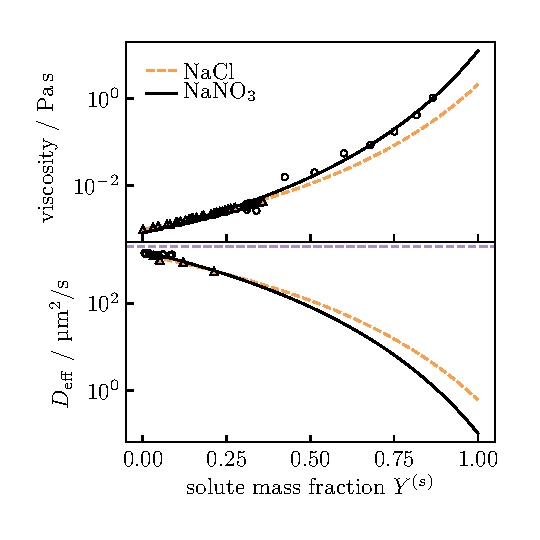
\includegraphics[width=0.9\linewidth,outer]{aerosol-diffusion-fit}
  \caption[Viscosity and diffusion coefficients of aqueous ionic solutions]{
    Numerical fits of binary diffusion coefficients for aqueous ionic solutions.
    a) fits of viscosity to an Arrhenius-like form \eqref{eq:vft-fit} to experimental values \cite{PowerCS2013,BaldelliAST2016}.
    b) diffusion coefficient from the viscosity fits assuming a Stokes-Einstein form \eqref{eq:stokes-einstein}, where the Stokes radius is obtained by calibration with direct measurements of diffusion at \SI{300}{\kelvin} for \ce{NaCl} \cite{LyubartsevJPC1996} and \SI{25}{\celsius} for \ce{NaNO3} \cite{YehJCED1970}.
    The dashed-purple horizontal line shows the diffusion constant of pure \ce{H2O} for reference, to be distinguished from the binary diffusion constants in the limit $Y^{(s)} \to 0$.}
  \label{fig:diffusion-fit}
\end{SCfigure}

We employ two simplifications in our calculations concerning the effects of droplet temperature.
First, our volume additivity assumption \eqref{eq:volume-additivity} makes the density temperature independent; this neglects conduction forces caused by temperature gradients and results in more heterogeneous droplets.
%In reality temperature gradients will be present in a drying droplet from evaporative cooling, so conductive forces will help keep the solution well-mixed; we will thus overestimate the inhomogeneities of the concentration profile.
Secondly, we approximate $T \sim T_\infty$ in the Stokes-Einstein relation \eqref{eq:stokes-einstein}
This approximation neglects evaporative cooling which would slow diffusion, so overestimates the diffusion constant and will result in more heterogeneous droplets.
It is unclear \emph{a priori} which of these opposing effects dominates.
Note: later we model the droplet temperature $T$ explicitly for treating solvent evaporation and nucleation rates, but we have not incorporated this temperature into the diffusion constant.

\subsection{Droplet boundary conditions}

Initially the droplets are prepared in equilibrium, so they are well-mixed solutions and we can assume a uniform initial concentration profile.
At $t=0$ the humidity is reduced leading to evaporation of the solvent.
The evaporation rate determines the boundary conditions for the diffusion equation \eqref{eq:final-diffusion}.

Integrating the species continuity equation \eqref{eq:species-continuity} gives the total mass flow into the droplet (of each species) as
\begin{equation}\label{eq:integral-continuity}
  \frac{d m^{(i)}}{dt} =
  \int_{V(t)} \frac{\partial \rho^{(i)}}{\partial t} \, d V +
  \int_{\partial V(t)} \rho^{(i)} \, \vec{v}_{\partial V(t)} \cdot d\vec{S}
%  \qquad i \in \{f,s\}
\end{equation}
where $V(t)$ is the volume of the droplet at time $t$ and $\vec{v}_{\partial V(t)}$ is the velocity of the boundary, and the vectorial surface element $d\vec{S}$ points in the direction of the outer normal vector.
We assume the solute does not leave the droplet, so all mass flow at the boundary must be due to the solvent.
Inserting the diffusion equation \eqref{eq:final-diffusion} into \eqref{eq:integral-continuity} and applying Stokes' theorem gives
\begin{equation}
  \frac{d m^{(s)}}{dt}
  =
  \int_{\partial V(t)}
  \Big(
  \rho^{(i)} \vec{v}_{\partial V(t)} +
  D_\mathrm{eff} \vec{\nabla} \rho^{(s)}
  \Big)
  \cdot d\vec{S}
  = 0.
\end{equation}
For spherical droplets this gives the boundary condition
%% \begin{equation}
%%   \frac{d m^{(s)}}{dt}
%%   =
%%   4 \pi R^2
%%   \rho^{(s)}(R) \left(
%%   \frac{dR}{dt}
%%   + \frac{D_\mathrm{eff}}{\rho^{(s)}} \frac{\partial \rho^{(s)}}{\partial r}
%%   \right)
%% \end{equation}
%% so
\begin{equation}
  \left. \frac{\partial \rho^{(s)}}{\partial r} \right|_{r=R(t)}
  =
  -
  \frac{\rho^{(s)}}{D_\mathrm{eff}(R)}
  \frac{dR}{dt}.
\end{equation}
Assuming volume additivity \eqref{eq:volume-additivity} we can determine the radial evolution from mass conservation as
\begin{equation}\label{eq:radial-evolution}
  \frac{dR}{dt}
  =
  \frac{\dot{m}}{4\pi R^2 \rho^{(f)}_0}
\end{equation}
so we need a model of the evaporation rate $\dot{m} := \tfrac{dm^{(f)}}{dt}$ to close this system of equations.

We now derive the classical result for quasistatic droplet vaporisation, loosely following the exposition of standard texts e.g.\ Refs.\ \cite{Slattery1999, Sirignano2010}.
Relaxation in the vapour phase occurs much faster than inside the liquid droplet, so we can assume that the flows in the vapour phase are quasi-steady.
The time-derivative in the continuity equations \eqref{eq:species-continuity} and \eqref{eq:species-continuity-relative} thus vanishes leaving
\begin{subequations}
  \begin{align}
    \vec{\nabla} \cdot (\rho \vec{v})
    &=
    0
    \\
    \vec{\nabla} \cdot (\rho^{(i)} \vec{v}^{(i)})
    =
    \vec{\nabla} \cdot (\rho^{(i)} \vec{v} + \vec{j}^{(i)})
    &=
    0
    \qquad i \in \{f,g\}
    %% \frac{1}{r^2} \frac{d}{dr} \left(
    %% r^2 \rho u Y_i - r^2 D_V \frac{d(\rho Y_i)}{dr}
    %% \right)
  \end{align}
\end{subequations}
with the total mass continuity equation obtained by summing over both species in \eqref{eq:species-continuity} and using $\sum_i \rho^{(i)} = \rho$.
Assuming spherical symmetry we find that total mass conservation obeys
\begin{equation}\label{eq:vapour-mass-conservation}
  r ^2 \rho v
  =
  \textrm{constant}
  =
  -\frac{\dot{m}}{4\pi}
\end{equation}
with radial speeds $v = |\vec{v}|$ and $v^{(i)} = |\vec{v}^{(i)}|$.
Similarly, for the evaporating component we obtain the ordinary differential equation
\begin{equation*}\label{eq:quasistatic-vapour-species-conservation}
  r^2 \rho v Y^{(f)} - r^2 \rho D_v \frac{d Y^{(f)}}{dr}
  =
  -\frac{\dot{m}}{4\pi}
\end{equation*}
where we assumed Fickian diffusion for the relative flux term with $D_v$ as the effective binary diffusion constant for the vapour.
Using total mass conservation \eqref{eq:vapour-mass-conservation} we can rewrite this as
\begin{equation}\label{eq:vapour-ode}
  \frac{d Q}{dr} (Y^{(f)} - 1)
  - \frac{d (Y^{(f)} - 1)}{dr}
  = 0
\end{equation}
with
\begin{equation}\label{eq:vapour-ode-integration-factor}
  Q(r)
  =
  \frac{\dot{m}}{4\pi}
  \int_r^\infty  \frac{1}{\rho D_v (r')^2} \, dr'.
\end{equation}
Upon integration%
\marginfootnote{One way of doing this is to multiply through by the integrating factor $e^{-Q(r)}$.}
we find
\begin{equation*}
  (Y^{(f)}(r) - 1) e^{-Q(r)}
  =
  \textrm{constant}.
\end{equation*}
or
\begin{equation*}
  \frac{1 - Y^{(f)}(R^+)}{\displaystyle{1 - \lim_{r \to \infty}} Y^{(f)}(r)}
  =
  1 + B
  =
  e^{Q(R)}
\end{equation*}
where the superscript in $Y^{(f)}(R^+)$ indicates the mass fraction of the solvent component is taken on the vapour side of the boundary and we have defined the \emph{Spalding number} as
\begin{equation}\label{eq:spalding-number}
  B
  =
  \frac{
    \displaystyle{\lim_{r \to \infty}} Y^{(f)}(r) - Y^{(f)}(R^+)
  }{
    1 - \displaystyle{\lim_{r \to \infty}} Y^{(f)}(r)
  }.
\end{equation}
Upon reinserting the definition of $Q(r)$ \eqref{eq:vapour-ode-integration-factor} and rearranging we obtain 
\begin{equation*}
  \frac{dm^{(f)}}{dt}
  =
  \frac{
    4\pi \ln{(1 + B)}
  }{
    \int_r^\infty  \frac{1}{\rho D_v (r')^2} \, dr'
  }.
\end{equation*}
If we take $\rho = \rho_v$ and $D_v$ as constants in the vapour phase, then we obtain the classical result for quasistatic vaporisation as \cite{Slattery1999,Sirignano2010}
\begin{equation}\label{eq:quasistatic-vaporisation}
  \frac{dm^{(f)}}{dt}
  =
  4\pi \rho_v D_v R \ln{(1 + B)}.
\end{equation}
Matching the partial pressures of the solvent on either side of the boundary through the Clausius-Clapeyron relation gives% the molar fraction
\begin{equation}\label{eq:molar-fraction}
  %X^{(f)}(R^+) =
  %a_w \frac{p_{eq}}{p}
  p_f(R^+)
  =
  p_f(R^-)
  \exp{\left( \frac{L}{R} \frac{T - T_\infty}{T T_\infty} \right)}
\end{equation}
where $p_f(R^\pm)$ are the partial pressures on either side of the surface which we can convert to mass fractions assuming Raoult's law in the gas phase combined with experimental fits of the solvent activity \cite{CleggJPCA1998}.
%The mass fraction $Y^{(f)}(R^+)$ can then be obtained from $X^{(f)}(R^+)$.
%% Neglecting the effects of radiative heat transfer, the steady state heat flux through the droplet boundary in the steady state is \cite{KulmalaJAS1992,RovelliJPCA2016}
%% \begin{equation}
%%   \dot{Q}
%%   =
%%   %Q_R
%%   - h \frac{dm^{(f)}}{dt} + 4\pi R K (T - T_\infty)
%% \end{equation}
%% %where $Q_R$ is the excess heat flux of radiation over absorption,
%% where $h_v$ is the vapour enthalpy of the evaporating solvent, and $K$ is the thermal conductivity of the gas phase.
Finally, assuming a steady state heat flux through the boundary, and neglecting the radiative heat transfer and the droplet heat capacity, gives the temperature difference between the droplet surface and the ambient temperature as \cite{KulmalaJAS1992,RovelliJPCA2016}
\begin{equation}\label{eq:temperature-difference}
  T - T_\infty = \frac{L}{4\pi R K} \frac{dm^{(f)}}{dt}
\end{equation}
% $L = h_v - h_l$
where $L$ is the specific latent heat of vaporisation, and $K$ is the thermal conductivity of the vapour phase.
Together, Eqs.\ \eqref{eq:quasistatic-vaporisation}, \eqref{eq:spalding-number}, \eqref{eq:molar-fraction} and \eqref{eq:temperature-difference} form a complete set of equations that can be solved (numerically) to obtain the evaporation rate.

Typically the classic vaporisation rate equation \eqref{eq:quasistatic-vaporisation} requires semi-empirical corrections to treat more complex mass and heat transport phenomena at the boundary.
We introduce the \emph{Sherwood number} $\sherwood$ to correct the vaporisation rate giving
\begin{equation}\label{eq:sherwood-correction}
  \frac{dm^{(f)}}{dt}
  =
  2\pi \, \sherwood \, \rho_v D_v R \ln{(1 + B)}.
\end{equation}
As a simplification we approximate $\sherwood$ as a constant throughout the droplet's trajectory and determine it by fitting the initial value of $\tfrac{dR}{dt}$ to the experiments.
At constant vaporisation rate the solution to the radial evolution equation \eqref{eq:radial-evolution} yields
\begin{equation}
  R(t)^2
  =
  R(t=0)^2
  + \left(2R \, \frac{dR}{dt}\right)_{t=0} t,
\end{equation}
valid at short times.
Fitting the early part of the experimental trajectory gives the initial $\tfrac{dR}{dt}$ and thus $\sherwood$ through \eqref{eq:sherwood-correction}.

\subsection{Implementation and results}

\begin{SCfigure}
  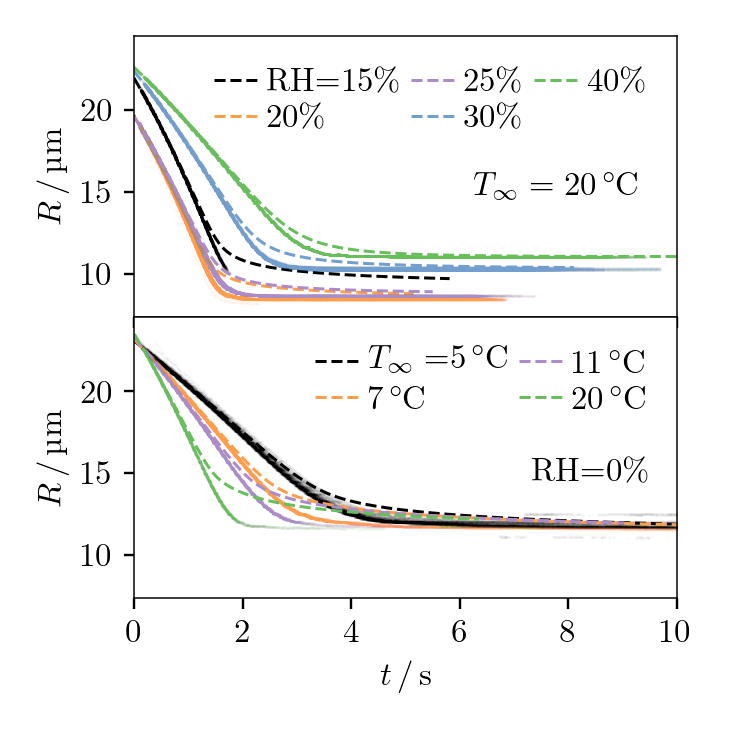
\includegraphics[width=0.9\linewidth,outer]{nano3-trajectory}
  \caption[Evolution of drying droplet radii]{
    Evolution of \ce{NaNO3} aerosol droplet radii from the numerical model (dashed lines) and experiments shown by points with 1\% transparency, showing reasonable agreement at short times until longer times when the evaporation rate is underestimated.
    a) varying relative humidity while ambient temperature is kept fixed, for an initial solute mass fraction of $Y^{(s)} = 0.125$.
    b) varying ambient temperature while relative humidity is kept fixed, for an initial solute mass fraction of $Y^{(s)} = 0.2$.}
  \label{fig:nano3-trajectory}
\end{SCfigure}

We discretise the solute concentration profile $\rho^{(s)}(r)$ onto a uniformly spaced grid over $r \in [0, R(t)]$.
To handle the moving boundary it is convenient to work in the rescaled coordinate $\tilde{r} = \frac{r}{R(t)} \in [0, 1]$.
For the discretisation we define the vector $\vec{\rho} := \{\rho_0, \rho_1, \cdots, \rho_N\}$ where $\rho_i := \rho^{(s)}\left(\tilde{r} = \frac{i}{N}\right)$.
The complete history of the evolution of the droplet then involves both $\vec{\rho}$ and $R$ variables.
In addition, it is convenient to introduce $\dot{R}$ as its own variable so that the final Jacobian for the diffusion equation \eqref{eq:final-diffusion} has tridiagonal form.
This gives us the evolving droplet state variable $\vec{x} = (\vec{\rho}, R, \dot{R})$.

To integrate a timestep $\Delta t$ we use the Crank-Nicolson \cite{CrankMPCPS1947} method where
\begin{equation*}
  \frac{\vec{x}(t + \Delta t) - \vec{x}(t)}{\Delta t}
  =
  \frac{1}{2}
  \left(
  \left. \frac{\partial \vec{x}}{\partial t} \right|_{t + \Delta t}
  +
  \left. \frac{\partial \vec{x}}{\partial t} \right|_t
  \right)
  + \mathcal{O}(\Delta t^2).
\end{equation*}
As the evolution equations are nonlinear this must be solved iteratively to find a self-consistent solution.
Introducing the $k$th approximation for $\vec{x}(t + \Delta t)$ as $\vec{x}^{(k)}(t + \Delta t)$, we write the next term in the sequence as $\vec{x}^{(k+1)} = \vec{x}^{(k)} + \delta \vec{x}^{(k)}$
We obtain
\begin{equation*}
  \frac{\vec{x}_{n+1}^{(k)} + \delta\vec{x}_{n+1}^{(k)} - \vec{x}_n}{\Delta t}
  =
  \frac{1}{2}
  \left(
  \frac{\partial (\vec{x}_{n+1}^{(k)} + \delta\vec{x}_{n+1}^{(k)})}{\partial t}
  +
  \frac{\partial \vec{x}_n}{\partial t}
  \right)
\end{equation*}
using the subscript $n$ as shorthand for the time.
This is a matrix equation that can be inverted for $\delta \vec{x}^{(k)}$.
Convergence is deemed to occur where $\delta \vec{x}^{(k)}$ falls below some threshold value.
The main advantage of this scheme over more simple schemes (e.g. forward Euler method where just the initial $\frac{\partial \vec{x}_n}{\partial t}$ is taken) is that the error is of order $\Delta t^2$ ensuring rapid convergence with small timesteps.

We integrated initially homogeneous droplets of \ce{NaCl} and \ce{NaNO3} for various ambient conditions.
The resulting radius , illustrated for \ce{NaNO3} in Fig.\ \ref{fig:nano3-trajectory}; we see that at short times there is excellent agreement, but the evaporation rate is underestimated at longer times.
This is likely do to limitations of the simplified evaporation model \eqref{eq:sherwood-correction} or because the neglect of conductive forces causes the evaporation to become diffusion-limited at long-times when the surface is highly enriched.
We achieve good agreement with experiments for \ce{NaCl} across their entire time-evolution (Fig.\ \ref{fig:nacl-trajectory}(b)) because these droplets crystallise before the slowdown of the evaporation rate.

\section{Nucleation model}
\label{sec:nucleation}

\subsection{Droplet nucleation rates}

\begin{SCfigure}
  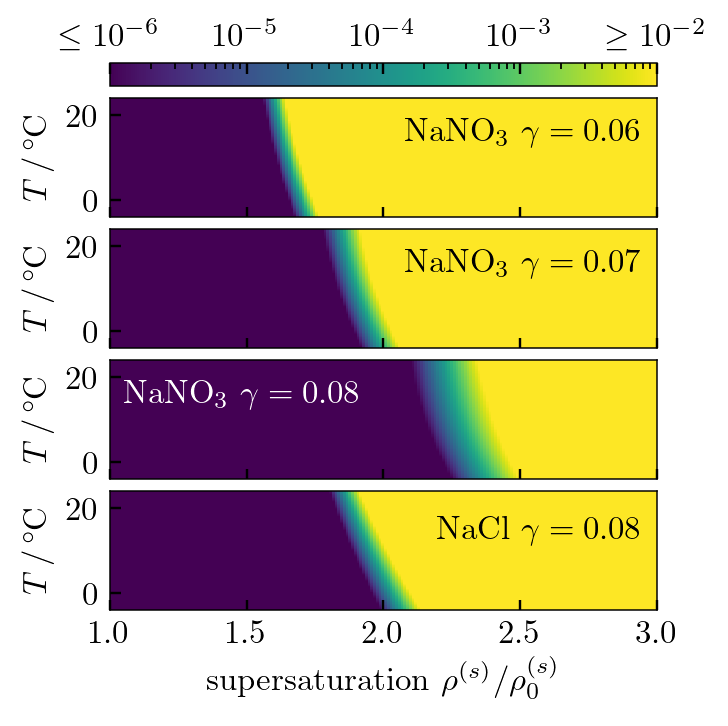
\includegraphics[width=0.9\linewidth,outer]{aerosol-cnt}
  \caption[Nucleation rates predicted by classical nucleation theory]{
    Shell nucleation rate $J\xi$ (\si{\per\micro\metre\squared\per\second}) predicted by classical nucleation theory for aqueous \ce{NaNO3} and \ce{NaCl} solutions at different state points.
    The dark blue and bright yellow regions show where nucleation is essentially impossible or instantaneous on the experimental timescale.
    Different estimates of solid-liquid surface tension $\gamma$ (given in \si{\newton\per\metre}) do not result in a different qualitative picture: a nucleation rate which monotonically increases with supersaturation and temperature.}
  \label{fig:cnt}
\end{SCfigure}

Denoting the rate of solute nucleation per unit volume as $J$, the continuum limit nucleation rate for the entire droplet is
\begin{equation}\label{eq:droplet-nucleation-rate}
  W
  =
  \int_V J dV
  =
  4\pi \int_0^R J(r) \, r^2 dr.
\end{equation}
Both the local $J$ and total rates $W$ contain an implciit time dependence because of their dependency on the evolving variables $R$, $\rho^{(s)}$ and $T$.
For homogeneous nucleation $J$ depends solely on the state variables $\rho^{(s)}$ and $T$.
Nucleation rates are typically strongly concentration dependent \cite{ValerianiJCP2005,DesarnaudJPCL2014,SearJPCM2007}, so we anticipate nucleation to occur at the boundary $r=R(t)$ where the solute concentration is greatest.
Allowing for heterogeneous nucleation $J$ could acquire an additional dependence on the inhomogeneities in the system; as the experiments were performed with high-purity precursor compounds to mitigate the effect of chemical impurities, we expect the main potential site for heterogeneous nucleation to be the liquid-air interface.
Whichever nucleation mechanism dominates, we expect it to occur at the boundary so the total rate \eqref{eq:boundary-nucleation-rate} reduces to
\begin{equation}\label{eq:boundary-nucleation-rate}
  W
  \sim
  4\pi R^2 J \xi
\end{equation}
where $J$ is now evaluated at the boundary, and we introduced $\xi$ as the thickness of the typical shell region over which nucleation occurs.
We will give nucleation rates in terms of $J \xi$, assuming a value $\xi = \SI{1}{\micro\metre}$ to set the absolute scale of the rates predicted by theory (section \ref{sec:cnt}) to most closely match the experiments.

We can relate the nucleation rates to the experimentally observed events by assuming Poisson statistics.
We define the survival probability as
\begin{equation*}
  p_\mathrm{liq}(t)
  :=
  \textrm{Prob}\left[ \textrm{no nucleation by time } t \right],
\end{equation*}
The mean number of nucleation events in the time interval $\Delta t$ is simply $W \Delta t$, giving the probability that there is no nucleation event after a time $\Delta t$ as
\begin{equation*}
  p_\mathrm{liq}(t + \Delta t) = p_\mathrm{liq}(t) e^{-W \Delta t}.
\end{equation*}
Taking the infinitesimal limit and using the fact that droplets are prepared in the liquid state giving the initial condition $p_\mathrm{liq}(t=0) = 1$ yields
\begin{equation}\label{eq:survival}
  p_\mathrm{liq}(t)
  =
  \exp{\left( -\int_0^t W \, dt \right)}.
\end{equation}
As we have already determined the droplet's radius and concentration profile from the evolution equations described in section\ \ref{sec:evolution}, we are left needing a model for the nucleation rate per unit volume $J$ before we can determine $p_\mathrm{liq}$.

\subsection{Nucleation models}
\label{sec:cnt}

%From \eqref{eq:cnt-barrier} we expect a homogeneous nucleation rate per unit volume as
For nucleation processes with a single barrier the rate per unit volume goes as
\begin{equation}\label{eq:nucleation-rate-barrier}
  J = \kappa \exp{\left(-\frac{\Delta G^{*}}{k_B T}\right)}
\end{equation}
where $\kappa$ is a kinetic prefactor and $\Delta G^*$ is thermodynamic barrier for the process.
A widely used approximation for the kinetic prefactor is \cite{SearJPCM2007}:
\begin{equation}
  \kappa = n_I j Z
\end{equation}
$n_I$ is the number density of potential nucleation sites, $j$ is the rate of aggregation to these sites, and $Z$ is the Zeldovich factor.
These last two quantities are typically further approximated as \cite{SearJPCM2007}
\begin{subequations}
  \begin{align}
    j &\sim n D_\mathrm{eff} R^* \\
    Z &\sim (N^*)^{-\tfrac{2}{3}}
  \end{align}
\end{subequations}
where $n$ is the solute number density, $N^*$ is excess number of molecules in the critical nucleus and $R^*$ is its radius.
The barrier $\Delta G^*$ depends on the specific nucleation mechanism.

For homogeneous nucleation the sites of nucleation are simply the solute molecules themselves so $n_I = n$.
The driving force for the transition is the chemical potential change $\Delta \mu$ from formation of the new phase.
In classical nucleation theory (CNT) the surface tension between the crystal and liquid is imagined as the main obstacle to nucleation.
Combining the two contributions leads to the barrier
\begin{equation}
  \Delta G = \gamma A - |\Delta \mu| n_c V
\end{equation}
where $n_c$ is the crystal number density, and $A, V$ are the surface areas and volumes of the nucleated region.
The thermodynamic barrier to nucleation is then the maximum of this formula; assuming a perfectly spherical crystal seed this gives
\begin{align}\label{eq:cnt-barrier}
  \Delta G^{*} &= \frac{4}{3} \pi (R^{*})^2 \gamma \\
  (R^{*}) &= \frac{2\gamma}{n_c |\Delta\mu|}.
\end{align}
The chemical potential expressed in terms of mean ionic activity is\cite{DesarnaudJPCL2014}
\begin{equation}
  %\exp{\left(
  \frac{\Delta \mu}{k_B T}
  %\right)}
  =
  2 \ln{\left( \frac{a_\pm}{a_{0\pm}} \frac{\rho^{(s)}}{\rho^{(s)}_0} \right)}
\end{equation}
where $a_\pm$ is mean ionic activity coefficient, $a_0$ is its value at saturation and $\rho^{(s)}_0$ is the threshold saturation concentration.

We find that CNT predicts homogeneous nucleation rates which increase monotonically in both concentration and temperature.
In Fig.\ \ref{fig:cnt} we show the predicted rates for \ce{NaCl} with $\gamma=\SI{0.08}{\newton\per\metre}$ and \ce{NaNO3} with different estimates of surface tension; we find that the rates increase so rapidly with concentration that they are essentially a step function over the timescale of the experiments.
This is qualitatively correct for \ce{NaCl}, so we are able to accurately predict the time of nucleation in the experiments shown in Fig.\ \ref{fig:nacl-trajectory}.
By contrast, the experiments show that the final survival probability for \ce{NaNO3} droplets is often in the range $0 < p_\mathrm{liq} < 1$ which is not consistent with nucleation rates being characterised by a step function, which we will make more quantitative in the next section.

\begin{SCfigure}
  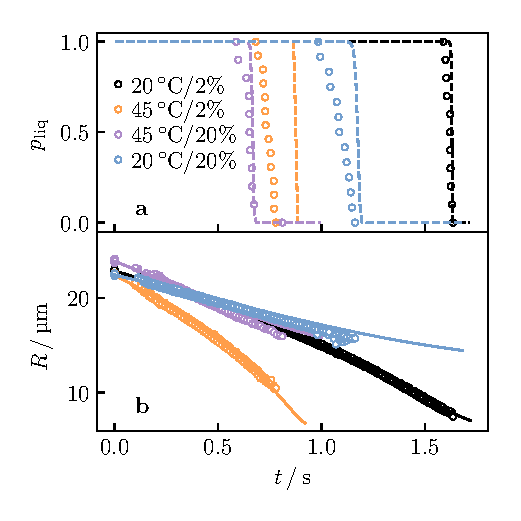
\includegraphics[width=0.9\linewidth,outer]{nacl-trajectory}
  \caption[Evolution of \ce{NaCl} droplets: theory and experiments]{
    Evolution of \ce{NaCl} droplets in dry air $\mathrm{RH}=0\%$ from experiments (points) and the numerical model (lines) for different ambient temperatures and initial solute mass fractions.
    a) the probability that a droplet survives without nucleating, assuming the liquid-crystal surface tension $\gamma = \SI{0.08}{\newton\per\metre}$ \cite{DesarnaudJPCL2014} for the numerical model.
    b) the evolution of droplet radius showing good treatment of solvent evaporation rates.
  }
  \label{fig:nacl-trajectory}
\end{SCfigure}

\subsection{Inferring nucleation rates from experiments}

We can try to determine the nucleation rates directly from experiments by observing the stochastic nucleation behaviour over repeat trajectories and comparing these against the numerical model.
The experiments give us the true survival probabilities $p_\mathrm{liq}$ of which we can determine the droplet nucleation rate $W$ exactly by numerical differentiation.
Combined with the numerical model, which gives us the precise state of the droplet, we can infer $J\xi$ from inversion of the rate formula \eqref{eq:boundary-nucleation-rate} under the assumption that nucleation is boundary-dominated.
%% We can make some progress by making some strong assumptions about the form of $J \xi$ based on physical intuition.
%% We will then test for self-consistency to justify this approach in an ad-hoc manner.

Differentiation of the survival probability \eqref{eq:survival} yields
\begin{equation}
  \dot{p}_\mathrm{liq}
  =
  - W p_\mathrm{liq},
\end{equation}
upon combining this with our assumption that nucleation occurs near the boundary \eqref{eq:boundary-nucleation-rate} allows to write the nucleation rate as
\begin{equation}
  J\xi
  =
  - \frac{1}{4\pi R^2} \frac{\dot{p}_\mathrm{liq}}{p_\mathrm{liq}}
\end{equation}
which we can determine from the experimentally observed $p_\mathrm{liq}$ trajectory.
The derivative of $p_\mathrm{liq}$ can be obtained through fitting.
The survival probabilities decay monotonically as a generalised step function, so we fit the experimental trajectories with the Fermi-Dirac form
\begin{equation}
  p_\mathrm{liq}(t) - \lim_{t \to \infty} p_\mathrm{liq}(t)
  =
  \frac{1 - \lim_{t \to \infty} p_\mathrm{liq}(t)}{\exp{\left[\epsilon(t - t_s)\right]} + 1}
\end{equation}
where $t_s$ is the time at which saturation is reached $\rho^{(s)}(R) = \rho^{(s)}_0$, and introducing the fitting function
\begin{equation*}
  \epsilon(t)
  =
  \begin{cases}
    at + bt^2 - c / t & \; t > 0 \\
    - \infty & \; t < 0
  \end{cases}
\end{equation*}
subject to the constraint that the fitting parameters $a, b, c \in [0, \infty]$ to ensure that $p_\mathrm{liq}$ decreases monotonically from $p_\mathrm{liq}(t=0)=1$.

We perform this inversion procedure for the \ce{NaNO3} droplets in Fig.\ \ref{fig:state-points}(b).
The resulting nucleation rates show non-mononic behaviour, increasing to a maximum before decreasing to essentially zero over the duration of the experiment.
This results in a finite final survival probability $p_\mathrm{liq} > 0$, and starkly contrasts with the picture predicted by CNT where $p_\mathrm{liq}$ would remain close to unity for most of the experiment before sharply dropping to zero as all droplets reproducibly crystallise.

\begin{SCfigure}
  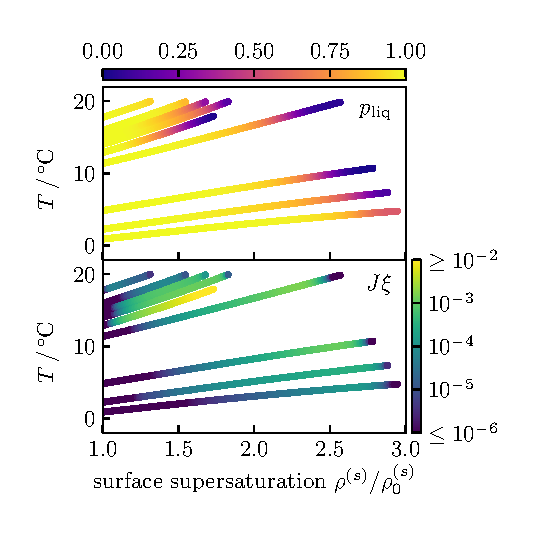
\includegraphics[width=0.9\linewidth,outer]{nano3-nucleation-rates}
  \caption[Experimentally observed nucleation rates in \ce{NaNO3} droplets]{
    State points explored by experiments with drying \ce{NaNO3}--\ce{H2O} aerosol droplets as determined from our numerical model for 9 datasets for different initial conditions.
    a) the survival probability in the experiments (i.e.\ the probability that a droplet has not crystallised), with state-point inferred from the model.
    b) the corresponding nucleation rates assuming boundary-dominated nucleation \eqref{eq:boundary-nucleation-rate} showing non-monotonic behaviour in increased concentration and temperature in contrast with the predictions of classical nucleation theory in Fig.\ \ref{fig:cnt}.}
  \label{fig:state-points}
\end{SCfigure}

\section{Conclusions}

We have developed a numerical model based on a diffusion equation with an extrapolation of the diffusion constant to high concentrations assuming the Stokes-Einstein relation.
The resulting droplet evolution conforms well to the experimental trajectories.
Assuming boundary dominated nucleation we are able to predict nucleation rates inside the droplet, and extract nucleation rates at differing state points from the experimental trajectories.

We found that CNT works well for predicting crystal nucleation in \ce{NaCl} but not \ce{NaNO3} aerosols.
In both cases CNT predicts nucleation essentially after a threshold surface saturation is reached, whereas experiments show nucleation in \ce{NaNO3} has stochastic behaviour.
This emerges from the fact that nucleation rates predicted by CNT monotonically increase in concentration and temperature.
In particular, the change in nucleation rate from increased concentration is so dramatic that the behaviour of CNT is essentially unchanged by small adjustments to the model parameters.

CNT is a model for homogeneous nucleation, so it is possible that it fails because crystallisation occurs for \ce{NaNO3} through heterogeneous nucleation.
The same stochastic phenomena are observed when repeating the experiments with the same droplet on a cycle of decreasing and increasing the RH to dry and melt the droplet; this rules out heterogeneous nucleation through impurities, as the chemical makeup is the same in each cycle yet the phenomenon persists.
This leaves the gas-liquid phase boundary itself as a site for hetereogeneous nucleation.

It is highly likely that the model overestimates the surface enrichment because at long times the simulated evaporation rates become limited by solute diffusion at the boundary.
The diffusion limit would persist even if more sophisticated transport phenomena were introduced to the evaporation model.
Surface enrichment is overestimated because we have neglected the effect of temperature gradients inside the droplet, and because we have used an extrapolation of low concentration diffusion data which likely to underestimate diffusion at high concentrations.
Temperature gradients create inward convection currents reducing surface enrichment.
Our extrapolation of the diffusion constant assumed the Stokes-Einstein relation holds across the whole state space, however this relation can be violated at high viscosities \cite{BerthierRMP2011}.
The rapid increase of viscosity with salt concentration in our model leads to a feedback loop where diffusion becomes increasingly difficult as the surface is enriched.
Correcting for these effects, we expect the surface concentrations explored by the experiments to increase to a maximum before decreasing which could explain non-monoticity.
However, this can only partially explain the observed behaviour because CNT is extremely sensitive to concentration.

%Our evaporation model considerably simplifies the transport phenomena at the phase boundary, though it becomes limited by the rate of solute diffusion at the boundary at long times suggesting that we are underestimating the rate of mixing.

%It is possible that our assumption that kinetics occurs purely through Fickian diffusion oversaturates the solute at the boundary, complicating our analysis of the nucleation rate.
%To go beyond this one would have to model temperature gradients to allow for conduction forces which help keep the droplet well-mixed.

This work is important in showing that the nucleation rate of nitrate aerosol is not only influenced by the level of supersaturation, but also by the drying kinetics itself because of an interplay between the inhomogeneity of the concentration profile and droplet temperature.
This is important for climate predictions where an understanding of the phase of atmospheric aerosol is crucial, and also valuable for spray-drying models where control over the resulting phase could be enabled by tuning the various drying parameters.

%% It is unlikely to be due to the trajectories being incorrect: even varying the most poorly estimated parameter for \ce{NaNO3}, the surface tension, does not change the CNT prediction.
%% Because of the sensitivity of CNT on parameters, it would require a remarkable degree of fine tuning to fit CNT model with any physically plausible parameters.
%% It's possible nucleation of \ce{NaNO3} occurs via a more complex kinetic pathway, e.g.\ multiple steps \cite{?,?,?}.
%% Alternatively, the experimental nucleation could be occurring via heterogeneous nucleation (e.g.\ impurities in the sample).
%% This is unlikely however, as the experiments can maintain the same salt sample and follow the single trajectory and it will still show the same stochastic behaviour.
%% Impurities are not likely to be in the solvent, or we would likely see the same phenomenon in \ce{NaNO3} nucleation.

%An option would be to relax the assumption that the temperature of the droplet is constant, as convection effects could play a key role in mixing the solution.
%Solving the Navier-Stokes equations would be essentially exact, though expensive route to include this.
%Less expensive would be to use vortex models or effective-conduction models which treat the internal circulation/convection of heat in an ad hoc manner.

\ifdefined\includebibliography
  \printbibliography
\fi

\end{document}
